\subsection{Fitting}

Given an observed time series, estimate which model best approximates its dynamics:\\
\begin{itemize}
    \item Choose from $\overbrace{AR(p),MA(q),ARMA(p,q),...}^\text{Model Selection}$ and estimate parameters (e.g., $\underbrace{\alpha_1,\ldots, \alpha_p, \beta_1,\ldots,\beta_q}_\text{estimation}$).
\end{itemize}

\textbf{\underline{Inference}}: Draw confidence intervals for parameters estimates \\

\textit{Note}: Inference for the mean of a stationary time series:\\

Let $X_t$ be a stationary time series. That means $E[X_t]=E[X_{t+1}]=E[X_{t+2}]=\ldots=\mu $. So $\mu$ is "population unconditional mean". Let $\gamma_k$ be the $k^{-th}$-order population autocovariance
\[
\gamma_k=Cov(X_t,_{t-k})
\]
Problem: Confidence interval for $\mu$ given $X_1,\ldots,X_T$

\begin{figure}[H]
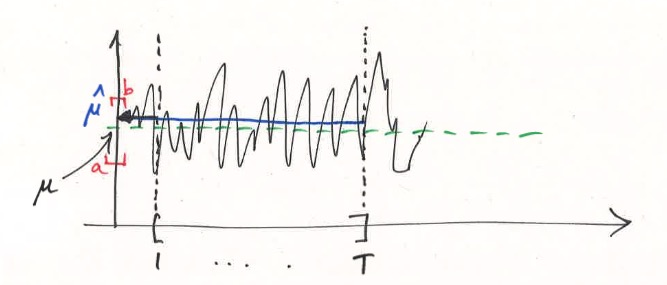
\includegraphics[scale=0.4]{images/Screenshot 2024-03-31 at 16.34.09.jpg}
\centering
\end{figure}

Regular stats confidence interval (margin of error measure): $\hat{\mu}=\frac{1}{T}\sum_{t=1}^T X_t=\bar{X}_T$\\

Want: C.I [a,b] s.t. $Pr(\mu$ in [a,b]$) \geq 95\%$ \\

\underline{Strategy}:

\begin{itemize}
    \item Calculate $var(\hat{\mu})=var(\bar{X}_T) $
    \item By Central Limit Theorem, $\Rightarrow \hat{\mu} \approx$ Gaussian
    \item Use 95\% quantiles of Gaussian with variance $var(\hat{\mu})$
    \item Produce a formula that can be coded and given to computer
\end{itemize}
Fact: If $\hat{\gamma}_k$ are sample analogues: do not use all of them for the sum because \begin{align*}
    \hat{var}(\hat{\mu}) &= \frac{1}{T}\sum_{t=1}^T var(X_t) + \frac{1}{T^2} \sum_{t\neq t} Cov(X_t, X_s) \\
    &= \frac{1}{T} T \hat{\gamma}_0 + \frac{1}{T^2} \sum_{s\neq t} \hat{\gamma}_k\\
    &= \hat{\gamma}_0 + \frac{1}{T^2} \sum_{k=1}^T \hat{\gamma}_k \cdot (T-k)
    &\text{vanishes $(=0)$ degrees of freedom problem}
\end{align*}
So instead, truncate at a given lag $h$. $l<<h<<T$ \quad Say \( \lfloor \sqrt{T} \rfloor \) or \( \lfloor log T \rfloor \)
\[
\hat{var}(\hat{\mu})=\frac{\hat{\gamma}_0}{1} + \frac{1}{T^2}\sum_{k=1}^h \hat{\gamma}_k (T-k)
\]
Then C.I $[a,b]=\hat{\mu} \pm 1.96 \sqrt{\hat{var}(\hat{\mu})} $
Sometimes called $\underbrace{\text{"HAC"}}_\text{heteroskedasticity, autocorrelation consistent}$ estimator

\begin{align*}
    var(\hat{\mu})&=var(\frac{1}{T}\sum_{t=1}^T X_t) \leftarrow \text{ difficult to expand if $Cov(X_t, X_s)\neq 0$}\\
    &=\frac{1}{T^2} \sum_{t=1}^T var(X_t) + \frac{1}{T^2} \sum_{s\neq t} Cov(X_t,X_s)\\
\end{align*}

usually with iid. data: would just estimate $\hat{var}(\hat{\mu})=\frac{1}{T}\sum_{t=1}^T(X_t-\hat{\mu})^2=\hat{\gamma}_0 $. Then form C.I.: $\hat{\mu}\pm 1.96 \times \hat{\gamma}_0^\frac{\sqrt{\hat{\gamma}_0}}{\sqrt{T}} $

\underline{In time series data}:
\begin{itemize}
    \item Can form $\hat{\gamma}_k$ for all $k$, and use it carefully
\end{itemize}


\subsection{PACF}

\underline{Partial Autocorrelation Function}, and choosing between $AR(p_1)$ and $AR(p_2)$ for 2 different Lags. \\

\textbf{\underline{Definition}}: \quad The function $PACF(k)$ is defined by the estimate $\pi_k$ in the least squares fit: \[
X_t=\nu +\pi_1 X_{t-1} +...+ \pi_k X_{t-k}
\]
In stats software packages, ---- bounds are drawn at $\pm \frac{2}{\sqrt{T}}$ like for auto correlation functions when properly normalized. This is done with unit variance scaling of $X_t$ (means replace $X_t$ with $\frac{X_t}{var(X_t)}=\frac{X_t}{\sigma^2}$)(Software does this automatically)

\begin{itemize}
    \item The PACF essentially isolated the direct effect of lag $k$ on the correlation, removing the influence of intermediate lags.
    \item This helps identify the order of AR terms in ARMA models. Significant spikes in the PACF at specific lags indicate potential AR components. A cut-off after lag $p$ in the PACF suggests an $AR(p)$ model might be appropriate
\end{itemize}

\subsection{Estimation}

Least squares estimation for $\varepsilon_t$ estimates. Note that least squares is equivalent to Maximum Likelihood for $\varepsilon_t$ Gaussian \\

For general $ARMA(p,q)$ model:

$ARMA(1,0)$: \[
X_t=\mu+\alpha X_{t-1} + \varepsilon_t+\beta\varepsilon_{t-1}
\]
\begin{itemize}
    \item Assume $\beta=0$ to start easy
    \item[] Given candidate $\alpha, \mu$ call it $\alpha^{\textit{candidate}}, \mu^{\textit{cand.}}$ Form: \[\hat{\varepsilon}(\alpha^{\textit{cand.}},\mu^{\textit{cand.}}) = X_t -\mu^{\textit{cand.}} - \alpha^{\textit{cand.}}X_{t-1}
    \]
    \item[] Calculate: \[SS(\alpha^{\textit{cand.}},\mu^{\textit{cand.}})=\sum_{t=2}^T \hat{\varepsilon}_t(\alpha^{\textit{cand.}},\mu^{\textit{cand.}} )^2 \]
    \item[] Take $\hat{\alpha}, \hat{\mu}$ to be minimizer of $SS(\alpha^{\textit{cand.}},\mu^{\textit{cand.}})$
\end{itemize}

Straight generalization to $MA(q)$ or $ARMA(p,q)$ etc. is \underline{not} straight forward.\\

\textbf{With MA}
\begin{itemize}
    \item $X_t=\mu+\varepsilon_t+\theta\varepsilon_{t-1}$ $\leftarrow$ Hard to do the instinctive thing, e.g.,
    \begin{itemize}
        \item[] $X_t-\mu-\varepsilon_t-\theta\varepsilon_{t-1}=0$
        \item[] $\underbrace{\varepsilon_t=X_t-\mu-\theta\varepsilon_{t-1}}_\text{Cannot square these and sum, because $\varepsilon_{t-1}$ is on inside.}$
        \begin{itemize}
            \item[] $\rightarrow$ Don't have an ex ante estimate $\hat{\varepsilon}_{t-1}$ \underline{unless} we approximate ("initialize") $\hat{\varepsilon}_0=0$
        \end{itemize}
    \end{itemize}
    \item For candidate $\mu^{\textit{cand.}}$, $\theta^{\textit{cand.}}$
    \begin{itemize}
        \item[]
        \begin{align*}
            \hat{\varepsilon}_1&=X_1-\mu^{\textit{cand.}}-\theta^{\textit{cand.}}\cdot \underbrace{\hat{\varepsilon}_0}_{=0}\\
            &=X_1-\mu^{\textit{cand.}}\\
        \end{align*}
        \item[]$\Rightarrow$ $\hat{\varepsilon}_1$ can be calculated now
        \begin{align*}
            \hat{\varepsilon}_2=X_2-\mu^{\textit{cand.}}-\theta^{\textit{cand.}} \cdot \hat{\varepsilon}_1
        \end{align*}
        \item[]$\Rightarrow$ $\hat{\varepsilon}_2$ can be calculated 
        \item[] etc.
    \end{itemize}
    \item[] Let $\hat{\mu}, \hat{\theta}$ $\underset{\mu^{\text{cand.}},\theta^{\text{cand.}}}{\text{minimize}}$ $\sum_{t=1}^T \hat{\varepsilon}_t^2$
    \begin{itemize}
        \item[] For finite order $MA(q)$, bias $\sim \frac{1}{T}$ is "small"
        \item[] ! This is smaller than $\frac{1}{\sqrt{T}}$, the statistical margin of error for $\hat{\mu}, \hat{\theta}$
    \end{itemize}
\end{itemize}

\textbf{General $ARMA(p,q)$ model:} Least Squares Approach
\[
X_t=\mu+\alpha_1X_{t-1}+...+\alpha_p X_{t-p}+\varepsilon_t+\theta_1 \varepsilon_{t-1}+...+\theta_q\varepsilon_{t-q}
\]
\begin{itemize}
    \item Initialize $\hat{\varepsilon}_0, \hat{\varepsilon}_{-1},...,\hat{\varepsilon}_{-q+1}=0 $
    \item[$\Rightarrow$] can calculate $\hat{\varepsilon}_1,\hat{\varepsilon}_2,...,\hat{\varepsilon}_T $ recursively, given candidate parameters
    \begin{itemize}
        \item Then minimize $\sum_{t=1}^T\hat{\varepsilon}_t^2 $
        \begin{itemize}
            \item[$\rightarrow$] $\hat{\mu},\hat{\alpha}_1,...,\hat{\alpha}_p, \hat{\theta}_1,...,\hat{\theta}_q $
        \end{itemize}
    \end{itemize}
    \item[] Can also minimize over $\hat{\varepsilon}_0$, computationally difficult 
\end{itemize}
\fbox{Maximum Likelihood Estimation} \quad (Alternative to Least Squares)
\begin{itemize}
    \item Native in Software
    \item Equivalent to Least Squares if $\varepsilon_t \sim N(0,\sigma^2)$, (i.e., $\varepsilon_t$ are Gaussian)
    \item Flexible enough that it can allow non-Gaussian $\varepsilon_t$ by appropriate adjustment to Likelihood
\end{itemize}

\subsection{Model Selection}

\begin{itemize}
    \item[] For $ARMA(p,q)$: \quad what should $p,q$ be?
    \item[] For $ARIMA(p,d,q)$: \quad what should $p,d,q$ be?
\end{itemize}
Guiding principle: Take $p+q0$ (or $p+d+q$) to be as small as possible while still modeling the data well
\begin{itemize}
    \item ACF and PACF of $\hat{\varepsilon}_t$ are zero (to statistical precision)
    \item Likelihood small relative to marginal benefit from the next parameter
\end{itemize}

\textbf{\underline{Tests for leftover correlation in residuals}}
\[
X_t=\hat{\mu} +\hat{\alpha}_1X_{t-1}+...+\hat{\alpha}_p X_{t-p}+\hat{\varepsilon}_t +\hat{\theta}_1\hat{\varepsilon}_{t-1}+...+\hat{\theta}_q \hat{\varepsilon}_{t-q}
\]
\begin{itemize}
    \item Look at ACF, PACF of $\hat{\varepsilon}_t$ against $\pm \frac{2}{\sqrt{T}}$ limits drawn by Software
    \item Ljung-Box test: For $\hat{r}_{\varepsilon,k}^2=$ autocorr. of $\hat{\varepsilon log k}$
    \begin{align*}
        Q&=T(T+2) \sum_{k=1}^K \frac{\hat{r}_{\varepsilon,k}^2}{T-k}\\
        Q &\sim \chi^2_{K-p-q} &&\text{d.f. $K$ choice, say $K=10$ e.g.}
    \end{align*}
    \begin{itemize}
        \item[] $H_0$: no serial correlation in residuals
    \end{itemize}
    \item Durbin-Watson test:
    \begin{align*}
        d&=\frac{\sum(\hat{\varepsilon}_t-\hat{\varepsilon}_{t-1})^2}{\sum (\hat{\varepsilon}_t^2)} \sim \text{ "DW", "Special reference dist."} \\
        &\approx 2(1-\hat{r}_{\varepsilon,2})
    \end{align*}
\end{itemize}

\textbf{\underline{Information Criteria}}
\begin{itemize}
    \item Akaike Information Criteria:
    \begin{itemize}
        \item $AIC=-2\cdot log\ Likelihood+2\cdot \# \ parameters$
    \end{itemize}
    \item Bias corrected Akaike Information Criteria 
    \begin{itemize}
        \item $AIC_c=-2\cdot log\ Likelihood + \frac{T\cdot 2\cdot \# parameters}{T-\#parameters-1}$
    \end{itemize}
    \item Bayesian Information Criteria:
    \begin{itemize}
        \item $BIC=-2\cdot log\ Likelihood+log\ T\cdot \# parameters$
    \end{itemize}
    \item[] Small $AIC$/$AIC_C$/$BIC$ preferred
    \begin{itemize}
        \item AIC under-penalizes relative to BIC:
        \begin{itemize}
            \item helpful for confidence intervals (for example $\hat{\alpha}_1\pm $ margin of error)
            \item Called under-smoothing - hoping less bias
        \end{itemize}
        \item BIC generally better for forecasting, $log\ T$ multiplier cancels typical boost in likelihood from added parameters
    \end{itemize}
\end{itemize}

